\documentclass[12pt]{spieman}  % 12pt font required by SPIE;
%\documentclass[a4paper,12pt]{spieman}  % use this instead for A4 paper
\usepackage{amsmath,amsfonts,amssymb}
\usepackage{graphicx}
\graphicspath{ {./figures/} }
\usepackage{setspace}
\usepackage{tocloft}
\usepackage{doi}

\newcommand{\code}[1]{\small \texttt{#1} \normalsize}

\title{Random Matrix Theory Tools for the Analysis of Functional Magnetic Resonance Imaging Examinations}

\author[a]{Derek Berger}
\author[a,*]{Jacob Levman}
\author[b]{Gurpreet M. Matharoo}
\affil[a]{St. Francis Xavier University, Department of Computer Science, 4130 University Avenue, Antigonish, Canada, B2G 2W5}
\affil[b]{St. Francis Xavier University, ACENET, 4130 University Avenue, Antigonish, Canada, B2G 2W5}


\renewcommand{\cftdotsep}{\cftnodots}
\cftpagenumbersoff{figure}
\cftpagenumbersoff{table}
\begin{document}
\maketitle

% \begin{abstract} This document shows the required format and appearance of a
% manuscript prepared for SPIE journals. It is prepared using LaTeX2e with the
% class file \texttt{spieman.cls}. Please note that the following journals
% require the use of structured abstracts in manuscript submissions:
% \textit{Neurophotonics}, the \textit{Journal of Biomedical Optics}, and the
% \textit{Journal of Medical Imaging}. Structured abstracts are encouraged for
% the \textit{Journal of Micro/Nanolithography, MEMS, and MOEMS}. Guidelines
% are available on the journal website. Whether structured or single-paragraph,
% the abstract should be a summary of the paper and not an introduction.
% Because the abstract may be used in abstracting and indexing databases, it
% should be self-contained (i.e., no numerical references) and substantive in
% nature, presenting concisely the objectives, methodology used, results
% obtained, and their significance. A list of up to six keywords should
% immediately follow. \end{abstract}

% See
% https://www.spiedigitallibrary.org/journals/journal-of-medical-imaging/volume-7/issue-01/010101/Integrating-structured-abstracts-in-the-Journal-of-Medical-Imaging/10.1117/1.JMI.7.1.010101.full
% for info on the structured abstract
%
% Purpose: This section presents the significance and aims, stating the broad
% impact and the rationale or motivation of the work, including potentially
% some background.
%
% Approach: This section briefly describes the materials and methods, including
% the statistical analyses, used in the research.
%
% Results: This section provides a core summary of the findings from the work,
% including study numbers, quantitative analyses, or discoveries.
%
% Conclusions: This section summarizes and interprets the approach and findings
% from the work, stating also the importance or impact of the findings.

% Purpose: Data-intensive modeling could provide insight on the broad
% variability in outcomes in spine surgery. Previous studies were limited to
% analysis of demographic and clinical characteristics. We report an analytic
% framework called “SpineCloud” that incorporates quantitative features
% extracted from perioperative images to predict spine surgery outcome.

% Approach: A retrospective study was conducted in which patient demographics,
% imaging, and outcome data were collected. Image features were automatically
% computed from perioperative CT. Postoperative 3- and 12-month functional and
% pain outcomes were analyzed in terms of improvement relative to the
% preoperative state. A boosted decision tree classifier was trained to predict
% outcome using demographic and image features as predictor variables.
% Predictions were computed based on SpineCloud and conventional demographic
% models, and features associated with poor outcome were identified from
% weighting terms evident in the boosted tree.

% Results Neither approach was predictive of 3- or 12-month outcomes based on
% preoperative data alone in the current, preliminary study. However,
% SpineCloud predictions incorporating image features obtained during and
% immediately following surgery (i.e., intraoperative and immediate
% postoperative images) exhibited significant improvement in area under the
% receiver operating characteristic (AUC): AUC=0.72 (CI95=0.59 to 0.83) at 3
% months and AUC=0.69 (CI95=0.55 to 0.82) at 12 months.

% Conclusions Predictive modeling of lumbar spine surgery outcomes was improved
% by incorporation of image-based features compared to analysis based on
% conventional demographic data. The SpineCloud framework could improve
% understanding of factors underlying outcome variability and warrants further
% investigation and validation in a larger patient cohort.
\begin{abstract}

\section*{Purpose}
Random matrix theory (RMT) is an increasingly useful tool for understanding
large, complex systems. Prior studies have examined functional Magnetic
Resonance Imaging (fMRI) scans using tools from RMT, with some success.
However, RMT computations are highly sensitive to a number of analytic choices,
and the robustness of findings involving RMT remain in question. We
systematically investigate the usefulness of RMT on a wide variety of fMRI
datasets using a rigorous predictive framework.

\section*{Approach}
We develop open-source software to efficiently compute RMT features from fMRI
images, and examine the cross-validated predictive potential of eigenvalue and
RMT-based features (``eigenfeatures'') with classic machine-learning
classifiers. We systematically vary pre-processing extent, normalization
procedures, RMT unfolding procedures, and feature selection, and compare the
impact of these analytic choices on the distributions of cross-validated
prediction performance for each combination of dataset binary classification
task, classifier, and feature. To deal with class imbalance, we use the
area under the receiver operating characteristic (AUROC) as the main
performance metric.

\section*{Results}
% df.groupby(["subgroup", "gross_feature"])["auroc"].median()
Across all classification tasks and analytic choices, we find eiegenfeatures to
more often have predictive utility than not (82.4\% of median AUROCs \(>\) 0.5;
median AUROC range across classification tasks 0.47 - 0.64). Simple baseline
reductions on source timeseries, by contrast, were less useful (58.8\% of
median AUROCs \(>\) 0.5, median AUROC range across classification tasks 0.42 -
0.62). Additionally, eigenfeature AUROC distributions were overall much more
right-tailed than baseline features suggesting greater predictive potential.
However, performance distributions were wide, and often significantly affected by
analytic choices.


\section*{Conclusions}
Eigenfeatures clearly have potential for understanding and reducing fMRI
functional connectivity. However, the utility of these features is strongly
dependent on analytic decisions, suggesting considerable caution when
interpreting past and future studies applying RMT to fMRI.

% This document shows the required format and appearance of a manuscript
% prepared for SPIE journals. It is prepared using LaTeX2e with the class file
% \texttt{spieman.cls}. Please note that the following journals require the use
% of structured abstracts in manuscript submissions: \textit{Neurophotonics},
% the \textit{Journal of Biomedical Optics}, and the \textit{Journal of Medical
% Imaging}. Structured abstracts are encouraged for the \textit{Journal of
% Micro/Nanolithography, MEMS, and MOEMS}. Guidelines are available on the
% journal website. Whether structured or single-paragraph, the abstract should
% be a summary of the paper and not an introduction. Because the abstract may
% be used in abstracting and indexing databases, it should be self-contained
% (i.e., no numerical references) and substantive in nature, presenting
% concisely the objectives, methodology used, results obtained, and their
% significance. A list of up to six keywords should immediately follow.
\end{abstract}

% Include a list of up to six keywords after the abstract
\keywords{random matrix, spectral rigidity, level number variance, fMRI, classification, machine-learning}

% Include email contact information for corresponding author
{\noindent \footnotesize\textbf{*}Jacob Levman,  \linkable{jlevman@stfx.ca} }

\begin{spacing}{2}   % use double spacing for rest of manuscript

\section{Introduction}
\label{sect:intro}  % \label{} allows reference to this section
% This document shows the format and appearance of a manuscript prepared for
% submission to an SPIE journal. Note that this template is only intended to be
% used as a guideline for author convenience. It is designed for optimum
% clarity and ease of reading for editors and reviewers, but the template does
% not reflect the final page layout of a published journal paper. Accepted
% papers are professionally typeset in XML according to the layout and design
% of the journal.


At its most rudimentary, RMT describes the expected behaviour of the
eigenvalues—also often called levels—of a number of classes of random
matrices\cite{andersonIntroductionRandomMatrices2010,
akemannOxfordHandbookRandom2011, mehtaRandomMatrices2004}. A random matrix is,
simplifying somewhat, a matrix in which the entries are drawn from
independently and identically distributed (\textit{iid}) distributions. Though
first developed to describe the fluctuation of nuclei energy levels in quantum
physics \cite{mehtaRandomMatrices2004, guhrRandommatrixTheoriesQuantum1998a},
RMT has been shown have extremely broad potential.

In small-scale physical systems, RMT universalities have been observed in
quantum chaotic systems, complex nuclei, atoms, molecules and disordered
mesoscopic systems
\cite{guhrRandommatrixTheoriesQuantum1998a,mehtaRandomMatrices2004,brodyRandommatrixPhysicsSpectrum1981,beenakkerRandommatrixTheoryQuantum1997,bohigasHigherOrderCorrelationsSpectra1985,wintgenLevelStatisticsQuantized1988,pandeySkewOrthogonalPolynomialsUniversality2001},
and at larger scales, RMT has been applied to atmospheric physics
\cite{santhanamStatisticsAtmosphericCorrelations2001}, stock cross-correlations
\cite{plerouRandomMatrixApproach2002} , social networks
\cite{jalanUncoveringRandomnessSuccess2014}, random networks
\cite{bandyopadhyayUniversalityComplexNetworks2007}, network-formation in
liquids
\cite{sastrySpectralStatisticsInstantaneous2001,matharooSpectralStatisticsQuenched2009}
and amorphous clusters
\cite{sarkarUniversalityVibrationalSpectra2004,matharooVibrationalSpectraAmorphous2005,matharooUniversalityVibrationalSpectra2008}.
Within biological systems, RMT has also been used to successfully model aspects
of  amino acid functional relationships
\cite{bhadolaTargetingFunctionalMotifs2016}, synchrony in epileptic seizures
\cite{osorioPhasesynchronizationRandommatrixBased2011}, and in protein-protein
interactions both in different species
\cite{agrawalQuantifyingRandomnessProtein2014} and breast cancer
\cite{raiRandomnessPreservedPatterns2015}. RMT has also been used to guide
statistical decisions in principal components
analyses\cite{franklinParallelAnalysisMethod1995,
veraartDenoisingDiffusionMRI2016, ulfarssonDimensionEstimationNoisy2008}, and,
even more recently, has provided insights into the behaviours of deep
neural networks\cite{martinImplicitSelfRegularizationDeep2021,
martinPredictingTrendsQuality2021}.

RMT likely has the most real-world explanatory potential when dealing with a
complex system of many (hundreds or more\cite{mehtaRandomMatrices2004})
interacting components. If such a system has a matrix representation, and the
eigenvalues of this representation have a distribution similar to one predicted
by RMT, it suggests the system is either highly random or chaotic. By contrast,
if the observed spectra deviate significantly from RMT-predicted spectra, this
suggests otherwise. A number of studies have used RMT to make such
interpretations and comparisons between
systems\cite{santhanamStatisticsAtmosphericCorrelations2001,
jalanUncoveringRandomnessSuccess2014,
bandyopadhyayUniversalityComplexNetworks2007,
agrawalQuantifyingRandomnessProtein2014, raiRandomnessPreservedPatterns2015,
sebaRandomMatrixAnalysis2003, wangSpectralPropertiesTemporal2015,
wangRandomMatrixTheory2016, matharooSpontaneousBackpainAlters2020}.

\subsection{RMT and Neurobiological Signals}

In the human brain, each neuron, collection of neurons, or region of interest
(ROI) is a potentially-interacting component in a highly complex system. RMT
may have potential in describing the totality of these interactions, provided
that measurements of functioning can be obtained with sufficient spatial and
temporal resolution to speak to some neurobiological or neuropsychological
phenomenon of interest.

For an imaging modality like fMRI, where changes in the
blood-oxygenation-level-dependent (BOLD) signals are related to neural
activity, RMT may be an ideal starting point. Each voxel time course (or
collection of such time sources - i.e. ROIs) can be considered an interacting
component of the system. Likewise, in \textit{functional connectivity}
analyses, statistical relationships of the BOLD ROI time-courses are
investigated in the hope of gaining insights into brain functioniong (see
\citenum{bastosTutorialReviewFunctional2016,
vandenheuvelExploringBrainNetwork2010} for reviews, but also
\citenum{nobleDecadeTestretestReliability2019} and
\citenum{lurieQuestionsControversiesStudy2020} for challenges facing functional
connectivity analyses). In this framework, each connection or correlation can
be considered a system component, and the eigenvalues of such a correlation
matrix can be examined from the perspective of RMT.

The earliest study taking this approach
demonstrated that spectra of the correlations between electroencephalographic
(EEG) signals closely resemble those of the Gaussian Orthogonal Ensemble (GOE)
\cite{sebaRandomMatrixAnalysis2003}. In fMRI, RMT has been used to
evaluate the quality of whole brain features extracted from fMRI data
\cite{voultsidouFeatureEvaluationFMRI2007,verganiRestingStateFMRI2019}, and in
diffusion MRI to aid in the selection of the number of
components to employ in principal-component reduction analysis and denoising
\cite{veraartDenoisingDiffusionMRI2016,verganiRestingStateFMRI2019,ulfarssonDimensionEstimationNoisy2008}.

RMT has also been used in ROI-based fMRI functional-connectivity studies to
investigate differences between rest and task states
\cite{wangSpectralPropertiesTemporal2015}, between subjects with and without
ADHD \cite{wangRandomMatrixTheory2016}, and between pain and non-pain states
\cite{matharooSpontaneousBackpainAlters2020}. Across these three studies, the
spectra of resting or low-attention states exhibited properties close to the
GOE. These findings suggest that certain aspects of psychological processes
might be characterized, in part, by features computed from the eigenvalues of
fMRI correlation matrices, and that these features might vary in an
interpretable manner across psychological processes. If this is the case, RMT
could aid in understanding the functioning of the human brain.


\subsection{Eigenvalues and Prediction}

The basic insight of RMT is thus that the eigenvalues alone may provide
interesting information about highly complex systems. However, real systems are
usually noisy, and involve a mixture of random and non-random components and
interactions. RMT is statistical in nature, describing only the expected
behaviour of the spectra of \textit{iid} random matrics. To this end, a number
of summary statistics or ``spectral observables''
\cite{mehtaRandomMatrices2004, guhrRandommatrixTheoriesQuantum1998a} can be
computed from empirically observed spectra, with these spectral observables
sometimes being better suited for further analysis, or for the comparison of
empirical observations to theory. Two such summary statistics that have been
popular\cite{santhanamStatisticsAtmosphericCorrelations2001,
jalanUncoveringRandomnessSuccess2014, matharooSpontaneousBackpainAlters2020,
bandyopadhyayUniversalityComplexNetworks2007,
agrawalQuantifyingRandomnessProtein2014, raiRandomnessPreservedPatterns2015,
sebaRandomMatrixAnalysis2003,wangSpectralPropertiesTemporal2015,
wangRandomMatrixTheory2016} are the \textit{spectral rigidity} and
\textit{level number variance} (``rigidity'' and ``level variance'' for short;
details in Section \ref{sect:methods}).

However, from a predictive standpoint, these summary statistics may eliminate
predictively-useful information. If the basic RMT insight is that the
eigenvalues alone can provide understanding of a system, then those eigenvalues
(or other simple transformations of them) ought also to be predictively
useful. We examine a number of such \textit{eigenfeatures} in this study.

In addition, the functional connectivity - the matrix of correlations of
various collections of voxels of an fMRI scan - is a priori a useful
representation of the fMRI data. However, the full correlation matrix between
all voxels is itself often computationally infeasible to work with, and thus is
reduced in various ways prior to being used in analyses.

Typical reductions include the use of a ``seed'' voxel or collection of voxels
(i.e. ROI): the mean signal over that ROI is correlated with all other N ROIs
of interest to generate a reduced functional connectivity matrix (or image)
with one correlation value at each non-seed ROI. This sort of reduction reduces
the functional connectivity to N values. This approach strongly biases the
analysis to the seed ROI.

Likewise, one can work with ROI mean signals, and work with the \(N \times N\)
matrix of these ROI correlations. This analysis [maybe cite Poldrack book for
this?] is, \textit{a priori}, sensitive to the choice of ROIs, and, in the case
of anatomical atlases / parcellations, may also lack theoretical justification.

A major disadvantage of both the above approaches, besides requiring
parcellation into ROIs, is that most such parcellation methods are atlas-based,
and thus require image registration, and, general, an entire preprocessing
pipeline to ensure that registration is successful.


RMT suggests a potentially useful reduction in the form of the eigenvalues of
the voxelwise functional connectivity. An \(N \times t\) matrix \(\bf{A}\) of
\(N\) time series of length \(t\), and where \(t \ll N\) will have a symmetric
correlation (or covariance) matrix with \(t - 1\) non-zero, positive
real-valued eigenvalues \(\Lambda\). These eigenvalues can be computed highly
efficiently via transposition of the voxelwise correlation or covariance
matrix.


\subsection{Limitations of Previous Work}

However, these previous studies took largely descriptive / explanatory
approaches, noting only differences in RMT across subgroups and/or conditions,
in many cases, with no formal statistical model nor formal testing of the
significance and robustness of these differences. No code was provided to allow
the reproduction of the results, and the extraction of the spectral rigidity
and level variance is non-trivial, and computationally demanding. Computation
of these spectral observables requires an \textit{unfolding}
procedure\cite{guhrRandommatrixTheoriesQuantum1998a,mehtaRandomMatrices2004},
which is, unfortunately, a poorly-documented fitting procedure that requires
making a number of difficult-to-justify decisions, and these decisions can
dramatically impact RMT conclusions
\cite{abul-magdUnfoldingSpectrumChaotic2014,abueleninSpectralUnfoldingChaotic2018,fossionRandommatrixSpectraTime2013,abueleninEffectUnfoldingSpectral2012,moralesImprovedUnfoldingDetrending2011}.
On top of the flexibility in the implementation and application of RMT to
empirical data, there is also the flexibility introduced by the choices in the
complex preprocessing pipelines of fMRI\cite{parkerBenefitSliceTiming2019}.

In addition these issues stemming from ``research degrees of freedom'' (cite
Gelman), there is also a basic baseline comparison issue: RMT is mathematically
non-trivial, the extraction of RMT spectral statistics is computationally
demanding, and eigenvalues, while easy to understand mathematically, are
difficult to interpret relative to simpler potential reductions of fMRI data.

What is missing is a rigorous, systematic, reproducible investigation of the
*predictice* value of RMT metrics across a wide variety of data, RMT analytic
choices, choice of eigenfeature, and choice of preprocessing, and for these RMT
eigenfeatures to be compared to simpler alternative baselines. The current
study aims to do just this.


\section{Datasets}
\label{sec:datasets}

\subsection{Overview}

We selected fMRI data publicly available on the
\href{https://openneuro.org/}{OpenNeuro} platform (36). Selection criteria was
somewhat subjective, but we required (1), that all scans have the same spatial
and temporal resolutions, (2), the the dataset comprise 10+ human subjects, and
(3), that it was reasonable to classify at the level of an entire scan, i.e.
neither task nor event timings were needed to determine class membership. This
yielded seven datasets comprising XX total subjects, and over 5000 total fMRI
volumes.


\begin{table}[h!]
\caption{
    ID = Identifier for paper. TR = Time of Repetition (seconds).
    Time = total duration (minutes) of each scan. Dimensions listed as M x N x P,
    indicate P horizontal / axial slices each with dimensions M x N.
}
\label{table:1}
\small
\centering
\begin{tabular}{ l c c c c c c }
\hline
\textbf{Name}    & \textbf{Dimensions}  & \textbf{Voxel size (mm)} & \textbf{TR} & \textbf{Volumes} & \textbf{n\_scans} \\
\hline
Aging     & 74 × 74 × 32   & 3.0 × 3.0 × 4.0 & 2.0  & 300 & 62  \\
Bilingual    & 100 × 100 × 72 & 1.8 × 1.8 × 1.8 & 0.88 & 823 & 90  \\
Depress   & 112 × 112 × 25 & 2.0 × 2.0 × 5.0 & 2.5  & 100 & 72  \\
Learn     & 64 × 64 × 36   & 3.0 × 3.0 × 3.0 & 2.0  & 195 & 432 \\
Osteo     & 64 × 64 × 36   & 3.4 × 3.4 × 3.0 & 2.5  & 300 & 74  \\
Park      & 80 × 80 × 43   & 3.0 × 3.0 × 3.0 & 2.4  & 149 & 552 \\
Attention & 128 × 128 × 70 & 1.5 × 1.5 × 1.5 & 3.0  & 300 & 90  \\
\hline
\end{tabular}
\end{table}

In order not to inundate readers with dataset details, and because this is an
exploratory investigation of RMT which is not committed to any specific
theory\footnote{In fact, datasets and, later, the classification tasks, were
chosen without investigation into any findings or publications associated with
the data, both in order to reduce bias in our decisions, and because the
original authors analytic / statistical approaches and intentions have very
limited relevance to our whole-brain, voxelwise, multiverse predictive
approach.}, we refer the reader to the original publications and/or data
releases when greater detail is needed, and highlight only the most basic
aspects of each dataset here.  Dataset scan parameters and acquisition details
are summarized in Table \ref{table:1}, and sample and subgroup sizes are
summarized in Table \ref{table:2}.

\begin{table}[h!]
\caption{
    ID = Identifier for paper. Subgroup = name of subgroup. Subjects = Number of subjects.
    Task = fMRI task. ANT = Attention Network Task \cite{fanActivationAttentionalNetworks2005}
}
\label{table:2}
\small
\centering
\begin{tabular}{ l r c c c }
\hline
\textbf{ID}  & \textbf{Subgroup}  & \textbf{Subjects}  & \textbf{Task} & \textbf{Scans per Subject} \\
\hline
Aging   &  older             & 28      & resting-state        & 1 \\
        &  younger           & 34      & resting-state        & 1 \\
        &                    &         &                      &   \\
Bilingual  &  bilingual          & 59      & resting-state    & 1 \\
        &  monolingual        & 33      & resting-state       & 1 \\
        &                    &         &                      &   \\
Depress &  depression         & 51      & resting-state       & 1 \\
        &  control            & 21      & resting-state       & 1 \\
        &                    &         &                      &   \\
Learn   &  task              & 24      & learn image sketches & 16\\
        &  rest              & 24      & resting-state        & 2 \\
        &                    &         &                      &   \\
Osteo   &  duloxetine        & 19      & resting-state        & 1 \\
        &  pain              & 37      & resting-state        & 1 \\
        &  nopain            & 20      & resting-state        & 1 \\
        &                    &         &                      &   \\
Park    &  Parkinson's       & 25      & ANT                  & 12\\
        &  control           & 21      & ANT                  & 12\\
        &                    &         &                      &   \\
Attention&  vigilant           & 11     & resting-state       & 2 \\
        &  nonigilant         & 11     & resting-state        & 2 \\
        &  trait-attentive     & 11    & resting-state        & 2 \\
        &  trait-non-attentive & 11    & resting-state        & 2 \\
        &  task-attentive     & 11     & resting-state        & 2 \\
        &  task-nonattentive  & 11     & resting-state        & 2 \\
\hline
\end{tabular}
\end{table}



\subsection{Datasets and Classification Tasks}


The \textit{Aging} dataset\cite{wahlheimIntrinsicFunctionalConnectivity2021}
included rs-fMRI data for 34 subjects with a mean age of 22 years (range: 18-32
years), and 28 subjects with a mean age of 70 years (range: 61-80 years). For
our analysis, we make the binary classification task the prediction of subject
age-group membership, i.e. \code{younger v older}.

% The final sample included 34 younger adults (1832 years old, Mage = 22.21, SD
% = 3.65; 20 female) and 28 older adults (61-80 years old, Mage = 69.82, SD =
% 5.64; 20 female). Table 1 shows that younger and older adults had comparable
% education and working memory capacity, the latter measured by forward and
% backward digit span (48). Older adults had higher vocabulary scores (49) and
% slower processing speed (50) than younger adults. Resting-state data
% comprised 300 measurements collected over one 10-minute run. This scan
% duration produces reliable functional connectivity estimates within and
% across participants (57). Participants were instructed to remain still and
% awake with their eyes open. No stimuli appeared during this scan, and the
% display was black. Functional scans were collected using an echo-planar image
% sequence sensitive to blood-oxygen-level-dependent (BOLD) contrast (T2*; 32
% slices with 4.0 mm thickness and no skip, TE = 30 ms, TR = 2000 ms, flip
% angle = 70, FOV = 220 mm, matrix size = 74 × 74 × 32 voxels, A/P phase
% encoding direction). Slices were collected in a descending order that covered
% the entire cortex and partial cerebellum. At the beginning of the
% resting-state scan, the scanner acquired and discarded two dummy scans.

% \subsubsection{Bilinguality Dataset}

The \textit{Bilinguality} dataset\cite{ds001747:1.0.0,
goldcarrieelizabethExploringRestingState2018} examined English and
Spanish-speaking monolinguals and multilinguals during a prolonged resting
state. The original study grouped participants into three subgroups: early vs
late bilinguals vs monolingual
controls\cite{goldcarrieelizabethExploringRestingState2018}. For our analysis,
we make the binary classification task be to classify \code{monolingual v
bilingual}.

% Resting state fMRI scans were performed using a T2*-weighted EPI sequence with the following
% parameters: TR=875ms; TE=43.6ms; slice thickness=1.8mm; acquisition matrix=100 × 100; flip
% angle=55°; number of slices=72; field of view=180 × 180mm; voxel size=1.8 × 1.8 × 1.8mm;
% multi-band factor=8; volumes per run=823 (total scan time=12min). EPI scans were oriented
% parallel to the long axis of the hippocampus.

% \subsubsection{Depression Dataset}

The \textit{Depression} dataset\cite{bezmaternykhddRestingStateClosed2021,
bezmaternykhBrainNetworksConnectivity2021} includes rs-fMRI scans frmo
non-depressed controls and mildy- or moderately-depressed subjects. The our analysis,
the binary classification task is \code{depress v control}.

% The intergroup study involved 21 healthy volunteers received a compensation
% for a participation and 51 participants featuring mild depression (F32.0),
% moderate depression (F32.1), or dysthymia (F34.1, single patient) (see Table
% 1). The fMRI study was carried out in the International Tomography Center,
% Novosibirsk, using a 3 T Ingenia scanner (Philips). Functional T2∗-weighted
% Ssh echo planar imaging scans were acquired using the following parameters:
% voxel size 2×2×5mm, repetition time/echo time = 2500/35 ms, and fat
% suppression mode. The reference anatomical image was obtained by the T1W 3D
% turbo field echo method with a voxel size of 1×1×1mm. The instruction for
% participants was to lie still with eyes closed for 6 minutes.

% \subsubsection{Learning Dataset}

The \textit{Learning} dataset\cite{schapiroHumanHippocampalReplay2018,
schapiroHumanHippocampalReplay2020} has both rs-fMRI and task fMRI scans were
available for all subjects, and \code{task v rest} is chosen as the binary
classification task for our analysis.  The task is complex and difficult to
summarize here adequately, but involved multiple phases where subjects were
presented with various related abstract images, and then later tested for their
memory of certain aspects of the learned images. Thus the classification task
might also be considered learning vs. rest.



% \subsubsection{Osteoarthritis Dataset}
The \textit{Osteo} dataset\cite{tetreaultBrainConnectivityPredicts2016}
includes whiole-brain rs-fMRI scans of healthy, pain-free controls
(\code{nopain} condition), and individuals with knee osteoarthritis.
Osteoarthritic patients were treated for 2 weeks with either placebo
(\code{pain} condition) or duloxetine (\code{duloxetine} condition).
We use the three binary classification tasks \code{nopain v duloxetine},
\code{nopain v pain}, and \code{pain v duloxetine} for our analysis.



% \subsubsection{Parkinson's Dataset}
The \textit{Park} dataset\cite{madhyasthaDynamicConnectivityRest2015} includes
subjects with non-demented Parkinson's Disease (PD) and
healthy controls performed a number of repetitions of the Attention Network
Task (ANT; \cite{fanActivationAttentionalNetworks2005}) during scans.
The classification task for this dataset is Parkinson's versus controls, i.e.
\code{park v ctrl}.

% \subsubsection{Attention Dataset}

The \textit{Attention} dataset\cite{gorgolewskiHighResolution7Tesla2015} is a
high-resolution rs-fMRI dataset including a battery of psychological measures
for each subject. Since previous studies employing RMT sometimes interpreted
their findings with respect to attentional processes
\cite{wangRandomMatrixTheory2016,matharooSpontaneousBackpainAlters2020}, we
divided subjects into various high vs. low attention binary classification
tasks based on median splits of subsets of the metrics available in this study.

The \code{viglant v nonvigilant} task was formed based on self-report
questionnaire items involving
"vigilance"\cite{gorgolewskiCorrespondenceIndividualDifferences2014}. The
\code{trait\_attend v trait\_nonattend} task was formed using PANAS-X
\cite{watsonPANASXManualPositive1994} items related to self-reported
wakefulness and attention over the past weeks. Finally, the
\code{task\_attend v tas\_nonattent} classification task was constructed
using the scores of The Conjunctive Continuous Performance Task
(CCPT\cite{shalevConjunctiveContinuousPerformance2011}). This is a behavioural
performance task which requires the subject to quickly and selectively respond
to only certain visual stimuli. Details allowing exact reproduction of these
splits are available in this paper's
\href{https://github.com/DM-Berger/random-matrix-fmri/blob/master/code/rmt/preprocess/unify\_attention\_data.py}{source
code}.



\section{Methods}
\label{sect:methods}

\subsection{fMRI Preprocessing}


We limited preprocessing to a simple pipeline of, in order, (1) brain
extraction, (2) slice timing correction, (3), motion correction, and (4),
registration to the MNI152
\cite{fonovUnbiasedAverageAgeappropriate2011,fonovUnbiasedNonlinearAverage2009}
2mm isotropic, asymmetric template version C made available through
\href{https://www.templateflow.org/}{TemplateFlow}
\cite{ciricTemplateFlowFAIRsharingMultiscale2021}.

We limited preprocessing methods to these steps sometimes because data required
for other typical preprocessing steps (e.g. field intensity maps, physiological
measurements), but also because we saved all pipelined intermediates to later
compare the effect of increasing degrees of pre-processing (see Section
\ref{sec:multiverse}), and it was important to limit the number of
preprocessing degrees to prevent excessive computational costs.

Brain extraction was performed first with BET
\cite{smithFastRobustAutomated2002}, and then with with
ANTs\cite{avantsReproducibleEvaluationANTs2011} to clean up residue left behind
by BET. BET results were visually inspected for each image in each dataset, and
BET fractional anisotropy values were modified to ensure brain extraction was
acceptable. Motion-correction was performed with FSL's MCFLIRT
\cite{jenkinsonImprovedOptimizationRobust2002}, and slicetime correction also
with FSL's \code{slicetimer}\cite{jenkinsonFSL2012} tool. Finally, functional
images were registered directly to the MNI152 template via
ANTs\cite{avantsReproducibleEvaluationANTs2011}.


\subsection{Feature Extraction}


For each preprocessing degree and fMRI image, features were extracted from all
\(N\) non-constant brain voxels, where \(N\) may differ for each image. After
this process, each scan yields an \(N \times T\) matrix \(\mathbf{M}\), where
\(T\) is the number of volumes acquired. All features summarize this matrix
of brain voxels \(\mathbf{M}\) in some manner.

\subsubsection{Raw Eigenvalues}
\label{sec:raw-eigs}

The time and space complexities of computing the full \(N \times N\) correlation
matrix of \(\mathbf{M}\), and the subsequent eigenvalues, are too large to be
tractable. However, since transposition does not change the eigenvalues, we
can use the transpose to efficiently compute these eigenvalues (see
Appendix \ref{sec:transpose}).




\subsubsection{RMT Features}
\label{sec:rmt-features}


To compare the observed eigenvalue distribution to some RMT theoretical
predictions, the eigenvalues must be unfolded
\cite{guhrRandommatrixTheoriesQuantum1998a,mehtaRandomMatrices2004}. The
details and motivation behind the unfolding procedure are well documented in
\cite{guhrRandommatrixTheoriesQuantum1998a}. Practically, the unfolding process
can be viewed as a smoothing and rescaling procedure where the originally
observed spectrum \(\lambda_1 \le \dots \le \lambda_n\) is smoothly mapped to
an unfolded spectrum \(e_1, \dots, e_n\), such that \(\sum d_i/n \approx 1\),
if \(d_i = e_{i+1} - e_i \). For most empirical data, the true smoothing
function is not known, and so must be approximated
\cite{guhrRandommatrixTheoriesQuantum1998a,mehtaRandomMatrices2004}. Typically,
a polynomial is chosen \cite{abul-magdUnfoldingSpectrumChaotic2014}.

Given empirically observed eigenvalues \(\Lambda\), the spectral rigidity,
\(\Delta_3(L)\), is calculated for any positive real value \(L <
\max(\Lambda)\) as:
\begin{equation}
\label{eq:rigidity}
\Delta_3(L) = \left \langle \min_{A,B} \frac{1}{L} \int_c^{c+L} \left(  \eta(\lambda) -A \lambda - B \right)^2 \right \rangle_c
\end{equation}
where \(\eta(\lambda)\) is the number of unfolded eigenvalues less than or
equal to \(\lambda\), \(\langle \cdot \rangle_c\) denotes the average with
respect to all starting points \(c\), and where \(A\) and \(B\) denote the
slope and intercept, respectively, of the least squares fit of a straight line
to \(\eta(\lambda)\) on \([c, c+L]\)
\cite{guhrRandommatrixTheoriesQuantum1998a}. Viewing the unfolded eigenvalues
as a timeseries, the spectral rigidty for a value \(L\) can be is thus the
\textit{average nonlinearity} of all intervals of length \(L\) over the series.


The level number variance, \(\Sigma^2(L)\), or level variance, for short, is
closely related to the spectral rigidity \cite{mehtaRandomMatrices2004}, and is
calculated as:
\begin{equation}
\label{eq:levlvar}
\Sigma^2(L) = \left\langle \eta^2(L, c) \right\rangle_c - \left\langle \eta(L, c) \right\rangle^2_c
\end{equation}
where \(\eta(L, c)\) is the number of unfolded eigenvalues in \([c, c+ L]\),
and where \(c\), \(L\), and \(\langle \cdot \rangle_c\) are as above
\cite{guhrRandommatrixTheoriesQuantum1998a}. Viewing the unfolded eigenvalues
as an \textit{irregular} timeseries, the level number variance is the
variation of the number of samples of all intervals of length \(L\) over the
series.

Both the spectral rigidity and level number variance are also computed and
investigated in this study, for all \(L \in \{ 1, 2, \dots 20 \}\).
Because the computation of these statistics is non-trivial, we developed and
release the separate, open-source Python library
\code{empyricalRMT}\cite{dm-bergerStfxecutablesEmpyricalRMTV12022}. The library
allows for efficient, parallel computation of the spectral rigidity and level
variance via Monte Carlo methods, and automatically ensures convergence of the
statistics to user-specified tolerances.

\textit{Trimming Variants}. As the unfolding procedure operates on the sorted
eigenvalues, and involves fitting a smooth polynomial or exponential to these
values, extreme values are often trimmed (or omitted from fitting)
\cite{moralesImprovedUnfoldingDetrending2011,
abueleninEffectUnfoldingSpectral2012}. The number of eigenvalues to trim is
highly subjective, and not usually well-documented. In addition, with a large
number of different source matrices, it is too destructive to use the same hard
criterion (e.g. largest 10\%, largest 3) for all unfoldings.

We develop and test four trimming variants: no trimming, precision-based,
largest, and middle, with far less subjective criteria for determining
trimming thresholds. However, we relegate the details of these trimming
procedures to the Appendix \ref{sec:trimming}, or refer readers to the \href{https://github.com/DM-Berger/random-matrix-fmri/blob/7c9e4187f582dedee728cd7193b8894d928c2f00/code/rmt/updated_dataset.py#L431-L444}{source code}.

\textit{Unfolding Variants}. Following any trimming, the eigenvalues are fit
with a polynomial. The choice of degree has been known to dramatically impact
certain analyses involving the spectral rigidity or level
variance\cite{abul-magdUnfoldingSpectrumChaotic2014,
moralesImprovedUnfoldingDetrending2011, abueleninSpectralUnfoldingChaotic2018,
fossionRandommatrixSpectraTime2013, abueleninEffectUnfoldingSpectral2012}. We
thus compute the rigidity and level variance with all possible combinations of
trimming and unfolding polynomial degree.

\subsubsection{Non-RMT Eigenfeatures}
\label{sec:eigs-only}

When computing the RMT eigenfeatures, the polynomial fitting during unfolding
has a smoothing effect, as do the additional averaging \(\langle\;\rangle_c\)
operations. However, it is possible other, simpler
transformations of the eigenvalues (e.g. uniform or Savitsky-Golay smoothing)
might have equal or greater predictive utility. We thus also test smoothed
variants of the eigenvalues as predictive features: we smooth the sorted
eigenvalues with a uniform (moving average) filter and Savitsky-Golay, using
window sizes of 3, 5, 7, and 9 to yield 8 total "smoothed eigenvalue" features.


\subsubsection{Slicing Variants}

We might expect the largest, middle, or smallest eigenvalues to be most useful
in characterizing some system. E.g. if the smallest eigenvalues correspond to
random / noise aspects of a system, but it is differences in the nature of the
noise that most differentiate between certain systems, then here the smallest
eigenvalues may have the most predictive utility.

Likewise, the \(L\) value in each RMT eigenfeature defines the degree of
locality at which we summarize the spectrum: at small \(L\)-values, the
spectral rigidity summarizes the non-linearity of eigenvalues that are
relatively close to each other in magnitude. At large values of \(L\), the rigidity
summarizes the long-range non-linearity of the spectrum.

Since predictive utility may vary with summary locality, or with the region of
the original spectrum, we investigate various front, middle, and end contiguous
slices of each eigenfeature in all analyses, where the size of each slice is
either the first or last 5\%, 10\%, or 20\% of the full eigenfeatures for
non-middle slices, or the middle 10\%, 20\%, or 40\% of the full eigenfeature for
the middle eigenvalues.

\subsubsection{Feature Combinations}

It could easily be the case that a combination of RMT and non-RMT eigenfeatures
are more predictive than either alone. We thus test a variety of eigenfeature
combinations, with the motivation for these particular combinations being to
test whether RMT eigenfeatures add anything beyond smoothing.
...




\subsubsection{Baseline Features}
\label{sec:baselines}

MAYBE MOVE THIS SECTION AFTER RMT AND EIGEN FEATURES?

If RMT- or eigenvalue-based features fail to predictively outperform features
that are simple summary statistics of the fMRI data, it is difficult to justify
the greater computational and interpretational complexities of the former. We
compute ten simple statistical reductions of the voxel time series ("timeseries
features") to help assess the relative value of RMT features.

Baseline reductions use as statistical summaries: robust measures of location
(mean, max, min); non-robust measures of location (median, \(95^{\text{th}}\)
percentile, \(5^{\text{th}}\) percentile); non-robust measures of scale
(standard deviation, range); and robust measures of scale (interquartile range,
difference between \(95^{\text{th}}\) percentile and \(5^{\text{th}}\)
percentile). These statistics are used to summarizing / reduce the fMRI data
along the voxel dimension, yielding a feature of \(T\) dimensions. E.g. the "mean"
feature is just the global mean signal. Exact details can be found in the
\href{https://github.com/DM-Berger/random-matrix-fmri/blob/master/code/rmt/enumerables.py#L51-L69}{paper
source code}. Note we do not take slice variants of these baseline features.

\subsubsection{Final Feature List}

[INSERT TABLE OF ALL FEATURES]


\subsection{Multiverse Analysis}
\label{sec:multiverse}

Our investigation can be structured hierarchically: we have a number of
\textit{datasets}, and each dataset has one or more \textit{classification
tasks}. Each classification task can be solved with a \textit{classifier}.
Each classifier fit operates on a \textit{featyre}, and each feature is
extracted via a certain \textit{preprocessing degree} and various
\textit{analytic choices} (slicing, trimming, unfolding degree, normalization).

\section{Results}
\label{sec:results}

\begin{figure}
\begin{center}
\begin{tabular}{c}
\includegraphics[width=6.5in]{gross_feature_overall_by_subgroup.png}
\end{tabular}
\end{center}
\caption
{ \label{fig:main-results}
AUROC distributions across gross feature groupings and comparison tasks.}
\end{figure}

First not non-predictable data, and then no longer discuss it in subsequent features.

\subsection{Normalization}
NO meaningful effect of normalization on AUROC distributions at level of gross feature, or feature
group, so can safely ignore this.
NO meaningful effect of normalization for any feature group by classifier either, so
normalization doesn't seem to matter here.
Maybe add table of correlations by groupings here

\subsection{Classifier}
When the data is predictable, timeseries features almost all have the mode / max <= 0.5 for all
classifiers and subgroups, whereas eigenfeatures (RMT, eigenvalue only, eigenvalue + RMT) more often
than not have mode greater than 0.5, and bulk of the distribution > 0.5.

KNN3 consistently has least favourable AUROC distributions across subgroups and features

\subsection{Page Setup and Fonts}

All text and figures, including footnotes, must fit inside a text area 6.5 in.\ wide by 9 in.\ high (16.51 by 22.86 cm). Manuscripts must be formatted for US letter paper, on which the margins should be 1 in.\ (2.54 cm) on the top, 1 in.\ on the bottom, and 1 in.\ on the left and right.

The Times New Roman font is used throughout the manuscript, in the sizes and styles shown in Table~\ref{tab:fonts}. If this font is not available, use a similar serif font. The manuscript should not contain headers or footers. Pages should be numbered.

\begin{table}[ht]
\caption{Fonts sizes and styles.}
\label{tab:fonts}
\begin{center}
\begin{tabular}{|l|l|} %% this creates two columns
%% |l|l| to left justify each column entry
%% |c|c| to center each column entry
%% use of \rule[]{}{} below opens up each row
\hline
\rule[-1ex]{0pt}{3.5ex}  Document entity & Brief description  \\
\hline\hline
\rule[-1ex]{0pt}{3.5ex}  Article title & 16 pt., bold, left justified  \\
\hline
\rule[-1ex]{0pt}{3.5ex}  Author names & 12 pt., bold, left justified   \\
\hline
\rule[-1ex]{0pt}{3.5ex}  Author affiliations & 10 pt., left justified   \\
\hline
\rule[-1ex]{0pt}{3.5ex}  Abstract & 10 pt.  \\
\hline
\rule[-1ex]{0pt}{3.5ex}  Keywords & 10 pt.  \\
\hline
\rule[-1ex]{0pt}{3.5ex}  Section heading & 12 pt., bold, left justified  \\
\hline
\rule[-1ex]{0pt}{3.5ex}  Subsection heading & 12 pt., italic, left justified  \\
\hline
\rule[-1ex]{0pt}{3.5ex}  Sub-subsection heading & 11 pt., italic, left justified  \\
\hline
\rule[-1ex]{0pt}{3.5ex}  Normal text & 12 pt. \\
\hline
\rule[-1ex]{0pt}{3.5ex}  Figure and table captions &  10 pt. \\
\hline
\end{tabular}
\end{center}
\end{table}

\section{Parts of Manuscript}

This section describes the normal structure of a manuscript and how each part should be handled. The appropriate vertical spacing between various parts of this document is achieved in LaTeX through the proper use of defined constructs, such as \verb|\section{}|.

\subsection{Title and Author Information}
\label{sect:title}
The article title appears left justified at the top of the first page. The title font is 16 pt., bold. The rules for capitalizing the title are the same as for sentences; only the first word, proper nouns, and acronyms should be capitalized. Do not begin titles with articles (for example, a, an, the) or prepositions (for example, on, by, etc.). The word ``novel'' should not appear in the title, as publication will imply novelty. Avoid the use of acronyms in the title, unless they are widely understood. Appendix A contains more about acronyms.

The list of authors immediately follows the title, 18 points below. The font is 12 pt., bold and the author names are left justified. The author affiliations and addresses follow the names, in 10-pt., normal font and left justified. For multiple affiliations, each affiliation should appear on a separate line. Superscript letters (a, b, c, etc.) should be used to associate multiple authors with their respective affiliations. The corresponding author should be identified with an asterisk, and that person's email address should be provided below the keywords.

\subsection{Abstract}
The abstract should be a summary of the paper and not an introduction. Because the abstract may be used in abstracting journals, it should be self-contained (i.e., no numerical references) and substantive in nature, presenting concisely the objectives, methodology used, results obtained, and their significance. Please note that the following journals require the use of structured abstracts in manuscript submissions: \textit{Neurophotonics}, the \textit{Journal of Biomedical Optics}, and the\textit{ Journal of Medical Imaging}. Structured abstracts are encouraged for the \textit{Journal of Micro/Nanolithography, MEMS, and MOEMS}. Helpful guidelines for structured abstracts are available on the website of the journal.

\subsection{Subject terms/Keywords}
Keywords are required. Please provide 3-6 keywords related to your paper.

\subsection{Body of Paper}
The body of the paper consists of numbered sections that present the main findings. These sections should be organized to best present the material.

To provide transition elements in your paper, it is important to refer back (or forward) to specific sections. Such references are made by indicating the section number, for example, ``In Sec.\ 2 we showed...'' or ``Section 2.1 contained a description...'' If the word Section, Reference, Equation, or Figure starts a sentence, it is spelled out. When occurring in the middle of a sentence, these words are abbreviated Sec., Ref., Eq., and Fig.

At the first occurrence of an acronym, spell it out followed by the acronym in parentheses, for example, charge-coupled diode (CCD).

\subsection{Footnotes}
Textual footnotes should be used rarely to present important documentary or explanatory material whose inclusion in the text would be distracting.\footnote{Example of a footnote.} Due to problems with HTML display, use of footnotes should generally be avoided. If absolutely necessary, the footnote mark must come at the end of a sentence. To insert a footnote, use the {\verb|\footnote{}|} command.

\subsection{Appendices}
Brief appendices may be included when necessary, such as derivations of equations, proofs of theorems, and details of algorithms. Equations and figures appearing in appendices should continue sequential numbering from earlier in the paper.

\subsection{Disclosures}
Conflicts of interest should be declared under a separate header, above Acknowledgments. If the authors have no competing interests to declare, then a statement should be included declaring no conflicts of interest. For assistance generating a disclosure statement, see the form available from  the International Committee of Medical Journal Editors website: \linkable{http://www.icmje.org/conflicts-of-interest/}

\subsection{Acknowledgments}
Acknowledgments and funding information should be added after the conclusion, and before references. Include grant numbers and the full name of the funding body. The acknowledgments section does not have a section number.

\subsection{Data, Materials, and Code Availability}
Availability of data, materials, and/or code used in the research results reported in the manuscript may be declared under the heading ``Data, Materials, and Code Availability,'' following the Acknowledgments section. As relevant, provide specific access information or restrictions for data, materials, and computer code (i.e., links to repository access addresses with guidance on commercial or public access).

\subsection{References}
The References section lists books, articles, and reports that are cited in the paper. This section does not have a section number. The references are numbered in the order in which they are cited. Examples of the format to be followed are given at the end of this document.

The reference list at the end of this document is created using BibTeX, which looks through the file {\ttfamily report.bib} for the entries cited in the LaTeX source file.  The format of the reference list is determined by the bibliography style file {\ttfamily spiejour.bst}, as specified in the \\ \verb|\bibliographystyle{spiejour}| command.  Alternatively, the references may be directly formatted in the LaTeX source file.

For books\citenum{Lamport94,Alred03,Goossens97} the listing includes the list of authors (initials plus last name), book title (in italics), page or chapter numbers, publisher, city, and year of publication.  Journal-article references \citenum{Metropolis53,Harris06} include the author list, title of the article (in quotes), journal name (in italics, properly abbreviated), volume number (in bold), inclusive page numbers or citation identifier, and year.  A reference to a proceedings paper or a chapter in an edited book\citenum{Gull89a} includes the author list, title of the article (in quotes), conference name (in italics), editors (if appropriate), volume title (in italics), volume number if applicable (in bold), inclusive page numbers, publisher, city, and year.  References to an article in the SPIE Proceedings may include the conference name, as shown in Ref.~\citenum{Hanson93c}.

The references are numbered in the order of their first citation. Citations to the references are made using superscripts, as demonstrated in the preceding paragraph. One may also directly refer to a reference within the text, for example, ``as shown in Ref.~\citenum{Metropolis53} ...''  Two or more references should be separated by a comma with no space between them. Multiple sequential references should be displayed with a dash between the first and last numbers \citenum{Alred03,Perelman97,Lamport94,Goossens97,Metropolis53}.

\subsubsection{Reference linking and DOIs}
A Digital Object Identifier (DOI) is a unique alphanumeric string assigned to a digital object, such as a journal article or a book chapter, that provides a persistent link to its location on the internet. The use of DOIs allows readers to easily access cited articles. Authors should include the DOI at the end of each reference in brackets if a DOI is available. See examples at the end of this manuscript. A free DOI lookup service is available from CrossRef at \\\linkable{http://www.crossref.org/freeTextQuery/}. The inclusion of DOIs will facilitate reference linking and is highly recommended.

In the present LaTeX template, the author needs to add the DOI reference by including it in a ``note'' in the bibliography file, as shown in the file {\verb+report.bib+}, for example, \\ {\verb+note = "[doi:10.1117/12.154577]"+}. The DOI may be used by the reader to locate that document with the link: {\verb+http://dx.doi.org10.1117/12.154577+}.

\subsection{Biographies}
A brief professional biography of approximately 75 words may be provided for each author, if available. Biographies should be placed at the end of the paper, after the references. Personal information such as hobbies or birthplace/birthdate should not be included. Author photographs are not published.

\section{Section Formatting}
\label{sect:sections}
In LaTeX, a new section is created with the \verb|\section{}| command, which automatically numbers the sections. Sections will be numbered sequentially, starting with the first section after the abstract, except for the acknowledgments and references. (Note that numbering of section headings is not required, but the numbering must be consistent if used.) All section headings should be left justified.

Main section headings are in 12-pt. bold font, left-justified and in title case, where important words are capitalized.

Paragraphs that immediately follow a section heading are leading paragraphs and should not be indented, according to standard publishing style. The same goes for leading paragraphs of subsections and sub-subsections. Subsequent paragraphs are standard paragraphs, with 0.2-in (5 mm) indentation. There is no additional space between paragraphs. In LaTeX, paragraphs are separated by blank lines in the source file. Indentation of the first line of a paragraph may be avoided by starting it with \verb|\noindent|.

\subsection{Subsection Headings}
All important words in a subsection (level 1) header are capitalized. Subsection numbers consist of the section number, followed by a period, and the subsection number within that section, without a period at the end. The heading is left justified and its font is 12 pt. italic.

\subsubsection{Sub-subsection headings}
The first word of a sub-subsection is capitalized. The rest of the text is not capitalized, except for proper names and acronyms (the latter should only be used if well known). The heading is left justified and its font is 11 pt. italic.

\section{Figures and Tables}

\subsection{Figures}

Figures are numbered in the order in which they are called out in the text. They should appear in the document in numerical order and as close as possible to their first reference in the text. It may be necessary to move figures or tables around to enhance readability. LaTeX will attempt to place figures at the top or bottom of a page in which they are first referenced.

Figures, along with their captions, should be separated from the main text by  0.2 in.\ or 5 mm and centered. Figure captions are centered below the figure or graph. Figure captions start with the abbreviation ``Fig'' in front of the figure number, followed by a period, and the text in 10-pt. font. See Fig.~\ref{fig:example} for an example.

\begin{figure}
\begin{center}
\begin{tabular}{c}
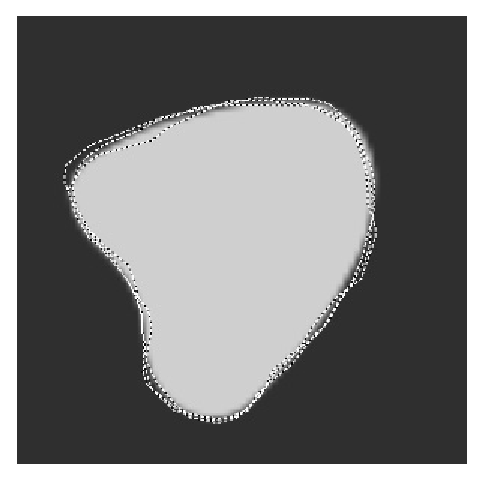
\includegraphics[height=5.5cm]{mcr3b.eps}
\end{tabular}
\end{center}
\caption
{ \label{fig:example}
Example of a figure caption. }
\end{figure}

Authors may wish to create figures consisting of two or more images, in which case, they should be neatly arranged in a rectangular array.  In no case, should the article's text be wrapped around a figure. Figure~\ref{fig:example2} shows two side-by-side images. When a figure contains more than one image, the author must submit them as a single image file. Further details about figure formatting can be found in the author guidelines for each specific SPIE journal: \\
\linkable {https://www.spiedigitallibrary.org/journals/journal-authors}.

\begin{figure}
\begin{center}
\begin{tabular}{c}

\includegraphics[height=5.5cm]{fig2.eps}  % fig2 includes two images
\\
(a) \hspace{5.1cm} (b)
\end{tabular}
\end{center}
\caption
{ \label{fig:example2}
Example of a figure containing multiple images: (a) sun and (b) blob. Figures containing multiple images must be submitted to SPIE as a single image file.}
\end{figure}

% \subsection{Tables}
% Tables are numbered in the order in which they are referenced. They should appear in the document in numerical order and as close as possible to their first reference in the text. It is preferable to have tables appear at the top or bottom of the page, if possible. Table captions are handled identically to those for figures, except that they appear above the table. See Table~\ref{tab:fonts} for an example.

% \subsection{Multimedia}
% Acceptable file formats, including MOV (.mov), MPEG (.mpg), and MP4 (.mp4), are playable using standard media players, such as VLC or Windows Media Player. The recommended maximum size for each multimedia file is 10-12 MB. Authors must insert a representative still image from the video file in the manuscript as a figure. The caption label will be linked by the publisher to the actual video file. The video may also be mentioned in an existing figure caption. Multimedia files are treated in the same manner as figures and they will be numbered sequentially with normal figures.  The video number, file type, and file size should be included in parentheses at the end of the figure caption. See Figure \ref{vid:satellite} for an example.

% \begin{video}
% \begin{center}
% {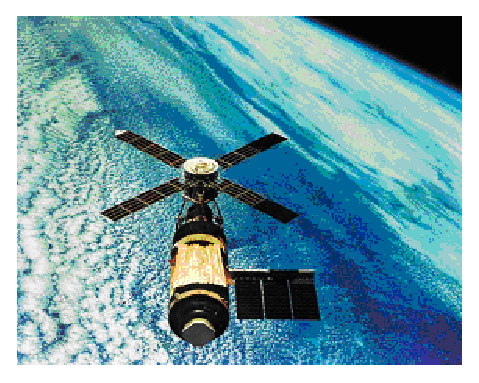
\includegraphics[height=5cm]{satellite.eps}}
% \\
% \end{center}
% \caption{\label{vid:satellite}This satellite is a still image from Video 1 (Video 1, MPEG, 2.5 MB).}
% \end{video}

\appendix    % this command starts appendixes

\section{Correlation Eigenvalues via Transposition}
\label{sec:transpose}

Let \(\mathbf{X}\) is a real \(n \times p\) matrix with \(n > p\). Let
\[
\mathbf{Z} = \text{norm}(\mathbf{X}) =
\left(
\mathbf{X}_1 - \bar{\mathbf{X}}_1 | \dots | \mathbf{X}_p - \bar{\mathbf{X}}_p
\right)
\]
where \(\mathbf{X}_i\) denotes column \(i\) of \(\mathbf{X}\). Denote the (unordered) set
of eigenvalues of \(\mathbf{X}\) as \(\text{eigs}(\mathbf{X})\), and let \(r = (p - 1)^{-1}\).
Denote the covariance matrix of \(\mathbf{X}\) as \(\text{cov}(\mathbf{X})\).  Then:

\begin{align*}
\text{eigs}\left( \text{cov}(\mathbf{X})  \right)
&= \text{eigs}(r \cdot \mathbf{Z}\mathbf{Z}^{\top}) \\
&= r \cdot \text{eigs}(\mathbf{Z}\mathbf{Z}^{\top}) \\
&= r \cdot \text{eigs}((\mathbf{Z}\mathbf{Z}^{\top})^{\top}) \\
&= r \cdot \text{eigs}(\mathbf{Z}^{\top}\mathbf{Z}) \\
\end{align*}

Denote the correlation matrix of \(\mathbf{X}\) as \(\text{corr}(\mathbf{X})\), and let
\[
\mathbf{Y} = \text{stand}(\mathbf{X}) =
\left(
(\mathbf{X}_1 - \bar{\mathbf{X}}_1) / \sigma_1 | \dots | (\mathbf{X}_p - \bar{\mathbf{X}}_p) / \sigma_p
\right)
\]

Then

\[
\text{eigs}\left( \text{corr}(\mathbf{X})  \right)
= \text{eigs}\left( \text{cov}(\mathbf{Y})  \right)
= r \cdot \text{eigs}(\mathbf{Y}^{\top}\mathbf{Y})
\]

\section{Trimming Procedures}

We implement three trimming procedures: precision-based, largest, and middle
trimming. The
\href{https://github.com/DM-Berger/random-matrix-fmri/blob/7c9e4187f582dedee728cd7193b8894d928c2f00/code/rmt/updated_dataset.py#L431-L444}{source
code} is the definitive reference for the procedures, but we describe the
motivations belows.

In precision-based trimming, we trim away any eigenvalues that are close enough
to zero to be considered a result of numerical error due to floating point
representation. There are two thresholds we consider, including the one used by
NumPy\cite{harrisArrayProgrammingNumPy2020} for the
\href{https://numpy.org/doc/stable/reference/generated/numpy.linalg.matrix_rank.html}{determination
of matrix rank}, and those recommended by LAPACK\cite{laug} in their user
guide\cite{andersonLAPACKUsersGuide1999a} on the
\href{https://netlib.org/lapack/lug/node89.html}{error bounds for symmetric
eigenproblems}, and related
\href{https://netlib.org/lapack/lug/node90.html}{additional details}. We trim
each matrix eigenvalues to whichever threshold is largest for the matrix in
question.

For largest trimming, we must determine a threshold at which to separate
"large" from "small" eigenvalues. The eigenvalues for our data tended to grow
exponentially, so we instead looked at thresholding on the logarithms. We then
used \(k\)-means with \(k=2\) on the precision-trimmed eigenvalues, and took
the largest cluster (which also always had the smaller mean) cluster as the
"largest" eigenvalues to trim away. "Middle" trimming simply reflects the
threshold found by the largest trim method, e.g. if the largest trim method
removes the last \(n\) precision-trimmed eigenvalues, then we also trim the
first \(n\) smallest eigenvalues remaining after precision-trimming.

We chose one-dimensional k-means partly due to efficiency and simplicity, and
because of the general relation to classical threholding methods like the Otsu
method\cite{liuOtsuMethodKmeans2009}.



% \section{Miscellaneous Formatting Details}
% \label{sect:misc}
% At times it may be desired, for formatting reasons, to break a line without starting a new paragraph. In a LaTeX source file, a linebreak is created with \verb|\\|.


% \subsection{Formatting Equations}
% Equations may appear inline with the text, if they are simple, short, and not of major importance; for example, $\beta = b/r$.  Important equations appear on their own line.  Such equations are centered.  For example, ``The expression for the field of view is
% \begin{equation}
% \label{eq:fov}
% 2 a = \frac{(b + 1)}{3c} \, ,
% \end{equation}
% where $a$ is the ...''  Principal equations are numbered, with the equation number placed within parentheses and right justified.

% Equations are considered to be part of a sentence and should be punctuated accordingly. In the above example, a comma appears after the equation because the next line is a subordinate clause. If the equation ends the sentence, a period should follow the equation. The line following an equation should not be indented unless it is meant to start a new paragraph. Indentation after an equation is avoided in LaTeX by not leaving a blank line between the equation and the subsequent text.

% References to equations include the equation number in parentheses, for example, ``Equation~(\ref{eq:fov}) shows ...'' or ``Combining Eqs.~(2) and (3), we obtain...'' Note that the word ``Equation'' is spelled out if it begins a sentence, but is abbreviated as ``Eq.'' otherwise. Using a tilde in the LaTeX source file between two characters avoids unwanted line breaks, for example between ``Eq.'' and the following equation number..

% \subsection{Formatting Theorems}

% To include theorems in a formal way, the theorem identification should appear in a 10-point, bold font, left justified, and followed by a period.  The text of the theorem continues on the same line in normal, 10-pt. font, achieved in LaTeX using \verb|\footnotesize|.  For example,

% \vspace{2ex}\noindent{\footnotesize\textbf{Theorem 1.} For any unbiased estimator...}

% \disclosures
\subsection*{Disclosures}
Conflicts of interest should be declared under a separate header. If the authors have no relevant financial interests in the manuscript and no other potential conflicts of interest to disclose, a statement to this effect should also be included in the manuscript.

\subsection* {Acknowledgments}
This unnumbered section is used to identify those who have aided the authors in understanding or accomplishing the work presented and to acknowledge sources of funding.

\subsection* {Data, Materials, and Code Availability}
As relevant, the availability of data, materials, and/or software code used in the research results reported in the manuscript may be declared in this section. (Note: this section is required for the \textit{Journal of Biomedical Optics} and \textit{Neurophotonics}.) Provide specific access information or restrictions for data, materials, and computer code (i.e., links to repository access addresses with guidance on commercial or public access).


%%%%% References %%%%%

\bibliography{report}   % bibliography data in report.bib
\bibliographystyle{spiejour}   % makes bibtex use spiejour.bst

%%%%% Biographies of authors %%%%%

\vspace{2ex}\noindent\textbf{First Author} is an assistant professor at the University of Optical Engineering. He received his BS and MS degrees in physics from the University of Optics in 1985 and 1987, respectively, and his PhD degree in optics from the Institute of Technology in 1991.  He is the author of more than 50 journal papers and has written three book chapters. His current research interests include optical interconnects, holography, and optoelectronic systems. He is a member of SPIE.

\vspace{1ex}
\noindent Biographies and photographs of the other authors are not available.

\listoffigures
\listoftables

\end{spacing}
\end{document}